\documentclass{article}

\usepackage{lmodern}
\usepackage{hyperref}
\usepackage{amsmath}
\usepackage{amssymb}
\usepackage[T1]{fontenc}
\usepackage{color,graphicx}

\begin{document}

\title{Kernel Based Approaches for Change-Point Detection \\ --- \\ Using penalized contrasts for the change-point problem. }
\date{May 21, 2016}
\author{Anirudhan J. Rajagopalan, ajr619}

\maketitle

\newpage

\section{Experiments for finding changepoints using spectral density}
We generate a sample time series signal which is a linear combination of four frequencies in the range of $\alpha, \beta, \delta, \theta $ frequencies.  We have also added some gaussian noise to the time series.

The timeseries is as given in figure~\ref{fig:cp_sd_ts}
\begin{figure}[ht!]
  \centering
  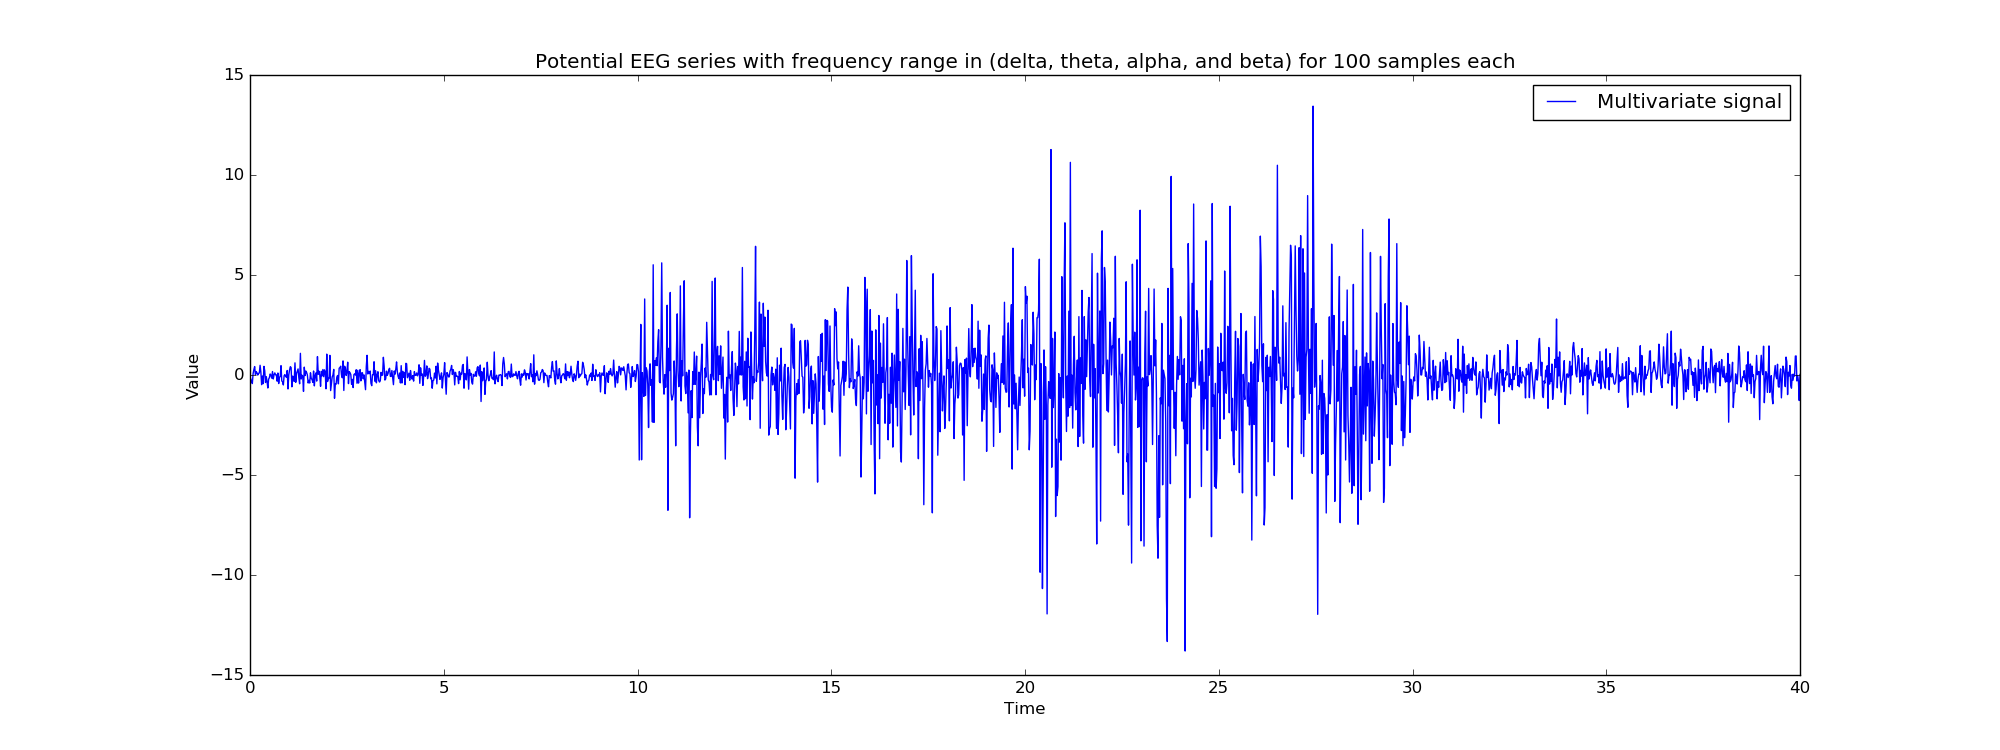
\includegraphics[width=1\textwidth]{images/changepoint_sd/ts}
  \caption{Time series formed by linear combination of sinusoidals with same frequency as that of brain signals.\label{fig:cp_sd_ts}}
\end{figure}

The data is sampled at 50 samples per second.

The code for finding the changepoints can be found in \url{https://git.io/vr2B3}.  The code consists of mainly three parts
\begin{enumerate}
  \item Contrast function
  \item Dynamic programming module to find the all possible change point paths.
  \item Model selection function that given a change point number, K, gives the indexes of change point in the time series data.
\end{enumerate}

The given timeseries has change points at point 500, 1000, 1500.  The algorithm gives change point values at \textbf{506, 985, and 1519}.

\bibliographystyle{plain}
\bibliography{references}

\end{document}
